\section{Metrics for evaluating predictions}

The following metrics can be used to analyze the quality of a \textit{classification model}.

\subsection{Confusion Matrix}

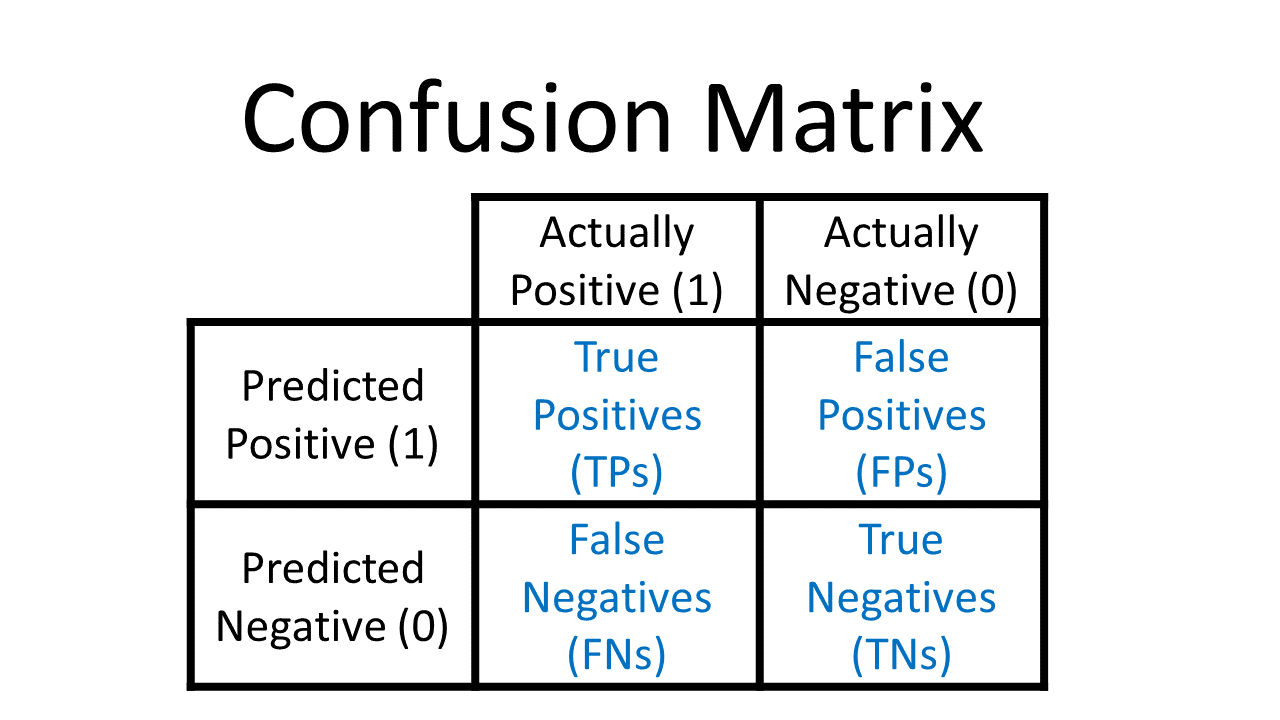
\includegraphics[width=400px]{confusion-matrix.png}

\subsection{Accuracy}

Accuracy answers the question \quotes{\textit{What is the probability that a prediciton is correct?}}.

$$
    Acc = \frac{TP + TN}{TP + TN + FP + FN}
$$

It is only good, if the real distribution of positive and negatives in the data is close to symmetric.

\subsection{Precision}

Precision answers the question \quotes{\textit{If we classify something as positive, how probable is it that it is actually positive?}}.

$$
    Precision = \frac{TP}{TP + FP}
$$

\subsection{Recall}

Recall a.k.a. sensitivity answers the question \quotes{\textit{If a sample is positive, what is the probability we also label it as positive?}}.

$$
    Recall = \frac{TP}{TP + FN}
$$

\subsection{F1 Score}

The F1-score divides the true positives by the sum of the true positives and the mean of the false positives and false negatives. This a high F1-score requires the model to make not few false predictions in either direction. Therefore F1-score is better than accuracy if the real distribution of positive and negative values in the dataset is uneven.

$$
    F1 = 2 \cdot \frac{Precision \cdot Recall}{Precision + Recall} = \frac{TP}{TP + \frac{1}{2} \cdot (FP + FN)}
$$


\section{One-hot encoding}

Many machine learning algorithms cannot have a categories as ouput values. Therefore if our goal is a categorization of samples we need to make a transformation of labels to numerical values.

\subsubsection*{Step 1: Integer Transformation}
First we must convert all different variants of the category into distinct integer values, e.g.:\\

\begin{tabular}{l l l}
    Dog         & $\rightarrow$ & 1 \\
    Cat         & $\rightarrow$ & 2 \\
    OtherAnimal & $\rightarrow$ & 3 \\
\end{tabular}

We can now train a machine learning model on that data and it will return one output value. To convert the models output back into classes we could pick the class where the ouput is the closest to the corresponding integer value.

\subsubsection*{One-Hot Encoding}

The problem with integer encoding is that we allow the model to that there is a defined order for the classes. E.g. in the above shown class mapping an ML model could assume that all other animals (3) are closer to cats (2) than to dogs (1). However, as this is not the case at all, using integer encoding might lead to poor predictions.\\
Instead we can use one-hot encoding resolving that issue. For each output class we create an output neuron / node with the value range of $[0, 1]$. The models predictions are converted back to the classes by taking the maximum of all values of the individual classes. The produces output for the individual classes can be seen as a probability that the sample is of instance of the corresponding class.

\begin{tabular}{l l l l l l}
    Dog         & $\rightarrow$ & $[0, 1]$ & $\longrightarrow$ &       \\
    Cat         & $\rightarrow$ & $[0, 1]$ & $\longrightarrow$ & $max$ \\
    OtherAnimal & $\rightarrow$ & $[0, 1]$ & $\longrightarrow$ &       \\
\end{tabular}

\section{Overfitting and Underfitting}

In supervised machine learning we usually have a function that determines a specific target parameter (e.g. if a passenger on the titanic survives). However, the function may not be accurate for all samples since the data may include errors (e.g. measurement errors). As we do not know the real underlying function we try to approximate it with supervised machine learning.\\
If a model is underfitted, it does not take all parameters of the real underlying function into account and therefore is not accurate.\\
If a model is overfitted, it takes parameters into account that do not apply to the underlying function but where given in the training samples. Overfitting leads to bad results on unseen data as parameters have been learned that are no general indicators for an event and can not be used on other data than the training samples. Overfitting may also occur if the paramters are tuned in a too detailed way that is only applicable to errors or inaccuracy of measurements in the training data.

\subsection{How can it be detected?}

To detect underfitting and overfitting we can validate the model after each training epoch by letting it make predictions on unseen data and calculating a chosen metric (in the figure we calculate a loss) over that data. Now we can make the following interpretations of the graph:

\begin{enumerate}
    \item As long as the loss is decreasing the model is still underfitted and shall be trained for more epochs.
    \item If the los is increasing the model is becoming more and more overfitted and training can be stopped.
    \item If the loss remains unchanged the model has reached the global or a local optimum.
\end{enumerate}

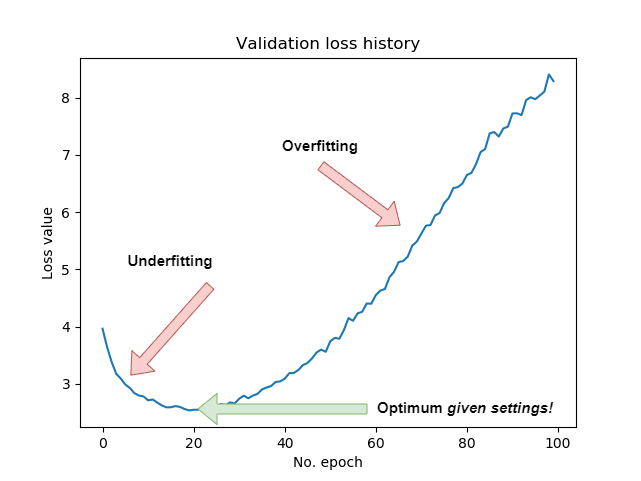
\includegraphics[width=400px]{underfitting-overfitting.png}

\subsection{Possible solutions}

\section{PCA - principal component analysis}

\subsection{Reasons for using PCA}
\subsection{Selection of good values for compon}

\section{Python Basics}

\subsection{Slicing}
\subsection{Data Extraction with Pandas}

\section{Regularization}
\subsection{What is regularization}
\subsection{Lasso}
\subsection{Ridge}
\subsection{Dropout}

\section{Machine Learning Tasks}

\subsection{Classification}
\subsection{Regression}
\subsection{Clustering}

\section{MLP - Multi-Layer-Perceptron}
\subsection{What is MPL?}
\subsection{Calculation of a number of parameters with and without bias}

\section{Feature map calculation in convolutional NN}

\section{Input and output sizes in Neural networks}
Describe here: Size of inputs and outputs in MLP and convolutional NN calculated from image size and the number of output classes.

\section{Activation functions}
\subsection{Softmax}
\subsection{Sigmoid}
\subsection{RELU}

\section{Solving non-linear problems with NNs}
Use example of logical function XOR here.

\section{K-means}

\section{Gradient Descent}

\section{Hyperparameters of ML models}

\subsection{Learning Rate}
\subsection{Epochs}
\subsection{Regularization}
\subsection{Batch Size}
\subsection{Convolution Kernel size}
\subsection{Max-Pooling}

\section{Logistic Regression and Cross Entropy}


\section{Linear Regression and Normal Equation}


\section{Decision Trees}


\section{K-nearest Neighbors}

